\subsection{Luminance stimulus construction}

The composition of the stimulus is a rather involved process, which can be separated in the following simpler steps:
\begin{enumerate}
    \item construction of the Gabor annulus with maximal contrast; \\
    First, a single annulus with maximal contrast is generated. To do this, we first compute the distance from the annulus center at every pixel. The pixels where this distance is smaller than the given radius of the annulus are assigned the corresponding luminance of the Gabor grating; others are assigned the designated void value. For more details, see Section \ref{sec:annulus-composition}.
    
    \item determining the position and coordinates of the figure in the stimulus; \\
    We start by selecting a random position of the figure within the stimulus given the figure size and its distance from the center of the stimulus. From there, the center of the figure, its coordinates, and the luminance matrix are computed. For more details, see Section \ref{sec:figure-composition}.
    
    \item positioning of the copies of the Gabor annulus in the stimulus; \\
    At this step, we first determine the distance between the neighboring annuli in the grid, which is equal to the number of pixels allocated to each annulus and void around it. Then, the number of annuli in each grid row and column is determined. Finally, the set of all annuli's coordinates is computed. For more details, see Section \ref{sec:annuli-locations}.
    
    \item assigning random contrasts to the different stimulus areas (figure, ground, void) depending on their location; \\
    First, the stimulus is initialized with the void luminance. Then, the annuli with relevant contrasts are added to the matrix at locations determined in the previous step. If annulus is located in the figure, its contrast is selected randomly from a small range of values, otherwise, from the larger range. For more details, see Section \ref{sec:luminance-assignment}.
    
    \item selecting a patch from the figure for further processing. For more details, see Section \ref{sec:patch-selection}.
\end{enumerate}

The result of completing the aforementioned steps includes a stimulus luminance matrix and a figure patch, examples of which are displayed in Figure \ref{fig:full-stimulus-example} and Figure \ref{fig:stim-patch-example}, respectively.

\subsubsection{Input parameters}
\label{sec:stimulus-parameters}

The appearance of the stimulus depends on many input parameters.
The reader may omit this section as the parameters are explained as they appear in the text. The summary list below is presented for convenience.

All spatial parameters are given in visual degrees: $1^\circ$ is equivalent to $1$ cm when the distance between the visual field and an eye is $37.5$ cm. For one such parameter (annulus diameter), the input is provided in pixels, too, allowing for scaling other parameters. The values given in visual degrees are further referred to as physical, and the pixel values - naturally, as pixel.

For the construction of an annulus, the following parameters are given:
\begin{itemize}
    \item $\spatfreq \in \mathbb{R}_+$ - the spatial frequency in cycles per degree;
    
    \item $\vlum \in [0, 1]$ - the void luminance value;
    
    \item $\diamdg \in \mathbb{R}_+$ - the diameter of a single annulus in visual degrees;
    
    \item $\diam \in \mathbb{N}$ - the diameter of a single annulus in pixels.
\end{itemize}
Since the mapping of the physical space (degrees) to pixel values in isomorphic, a conversion coefficient $\atopix \in \mathbb{R}_+$ between the two can be defined as follows:
\begin{equation}
    \atopix = \frac{\diam}{\diamdg}.
\end{equation}

The parameters relevant for the full stimulus are
\begin{itemize}
    \item $\anndistscale \in [1, \infty)$ - the scalar that represents the distance scale between neighboring annuli (the minimum possible value is $1$ to ensure the annuli do not overlap);
    
    \item $\fullwidthdg \in [\diam, \infty)$ - the width of the stimulus in visual degrees; in pixels, the width is
    $
        \fullwidth = \ceil{\atopix \cdot \fullwidthdg};
    $
    
    \item $\fullheightdg \in [\diam, \infty)$ - the height of the stimulus in visual degrees; in pixels, the height is
    $
        \fullheight = \ceil{\atopix \cdot \fullheightdg}.
    $
\end{itemize}

The parameters relevant for the figure are
\begin{itemize}

    \item $\contrange \in (0, 1]$ - the range of annuli contrasts in the figure;
    
    \item $\figwidthdg \in (0, \frac{1}{2} \fullwidthdg]$ - the width of the figure in visual degrees (must fit in the bottom right quadrant of the stimulus); in pixels, the width is
    $
        \figwidth = \ceil{\atopix \cdot \figwidthdg};
    $
    
    \item $\figheightdg \in (0, \frac{1}{2} \fullheightdg]$ - the height of the figure in visual degrees; in pixels, the width is
    $
        \figheight = \ceil{\atopix \cdot \figheightdg};
    $
    
    \item $\figeccdg \in [\figdiag, \| (\frac{1}{2} \fullwidthdg, \frac{1}{2} \fullheightdg)\| - \figdiag]$, where
    \begin{equation}
        \figdiag = \left\| 
            \left(
                \frac{1}{2} \figwidthdg, 
                \frac{1}{2} \figheightdg 
            \right)
        \right\|,
        \label{eq:figdiag}
    \end{equation}
    - the distance between the center of the stimulus and the center of the figure in visual degrees; in pixels, this distance is
    $
        \figecc = \ceil{\atopix \cdot \figeccdg}.
    $
\end{itemize}

Finally, the parameter for the stimulus patch is
\begin{itemize}

    \item $n \in \mathbb{N}$ - the number of PING networks in each dimension of the oscillatory network, as shown in Section \ref{sec:grid-network};
    
    \item $\patchsizedg \in (0, \min(\figwidthdg, \figheightdg)]$ - the side length of the stimulus patch in visual degrees; in pixels, the length is
    $
        \patchsize = \ceil{\atopix \cdot \patchsizedg}.
    $
    Additionally, for further processing, $(n | \patchsize)$ must hold.
\end{itemize}

The parameters' values used for composing the stimuli are displayed in Table \ref{tab:stimulus-composition-params}.

\begin{table}[!htp]
    \centering
    \begin{tabular}{|
>{\columncolor{main-color}}c |ccccc|}
\hline
\textbf{Parameter}      & \multicolumn{5}{c|}{\cellcolor{main-color}\textbf{Value(s)}}                                                                      \\ \hline
\textbf{$\pmb{\hat{d}}$}      & \multicolumn{5}{c|}{$0.7^\circ$}                                                                                                    \\ \hline
$\pmb{\vlum}$           & \multicolumn{5}{c|}{$0.5$}                                                                                                          \\ \hline
\textbf{$\pmb{\Omega}$} & \multicolumn{5}{c|}{$5.7$ cycles/degree}                                                                                            \\ \hline
$\pmb{\hat{\ell_{F_w}}}$      & \multicolumn{5}{c|}{$(9 \pm 0.7)^\circ$}                                                                                            \\ \hline
$\pmb{\hat{\ell_{F_h}}}$      & \multicolumn{5}{c|}{$(5 \pm 0.4)^\circ$}                                                                                            \\ \hline
$\pmb{\hat{\ecc_F}}$          & \multicolumn{5}{c|}{$(7 \pm 1)^\circ$}                                                                                              \\ \hline
$\pmb{k}$               & \multicolumn{1}{c|}{$1$}    & \multicolumn{1}{c|}{$1.125$}  & \multicolumn{1}{c|}{$1.250$}  & \multicolumn{1}{c|}{$1.375$}  & $1.5$ \\ \hline
$\pmb{\eta}$            & \multicolumn{1}{c|}{$0.01$} & \multicolumn{1}{c|}{$0.0257$} & \multicolumn{1}{c|}{$0.5050$} & \multicolumn{1}{c|}{$0.7525$} & $1$   \\ \hline
\end{tabular}
    \caption[Stimuli parameters]{The values of the parameters used to generate texture stimuli. The parameters are chosen to be either identical or close to \cite{MaryamPLACEHOLDER}.}
    \label{tab:stimulus-composition-params}
\end{table}
\subsubsection{Annulus composition}
\label{sec:annulus-composition}

Let $\annradii \in [0, 1]^{\diam \times \diam}$ be a matrix containing the distances (radii) of each pixel from the middle of the matrix. If $\diam = 1$,
\begin{equation}
    \annradii = 
    \begin{pmatrix}
        0
    \end{pmatrix}.
\end{equation}
Otherwise, for $i, j \in \{ 0, 1, \cdots,  \diam-1 \}$,
\begin{equation}
    \annradii_{i, j} = \left\| 
        (0, 0), \ 
        \left(
            -\frac{\diamdg}{2} + \frac{\diamdg}{\diam - 1} i, 
            -\frac{\diamdg}{2} + \frac{\diamdg}{\diam - 1} j 
        \right) 
    \right\|.
\end{equation}

Let $\annmatrix \in [0, 1]^{\diam \times \diam}$ be the pixel luminance matrix of the annulus. Then, for $i, j \in \{ 0, 1, \cdots,  \diam-1 \}$,
\begin{equation}
    \annmatrix_{i, j} = \vlum \cdot
    \begin{cases}
        \cos(2 \pi \annradii_{i, j} \spatfreq + \pi) 
        &\text{ if } \annradii_{i, j} \leq \frac{\diamdg}{2} \\
        1 
        &\text{ otherwise}
    \end{cases},
    \label{eq:grating}
\end{equation}
where $\vlum \in [0, 1]$ is luminance of the void (the area uncovered by the annulus).
An example of the resulting luminance matrix' binary heat map is visualized in Figure \ref{fig:grating-example}.

\begin{figure}[!htp]
    \centering
    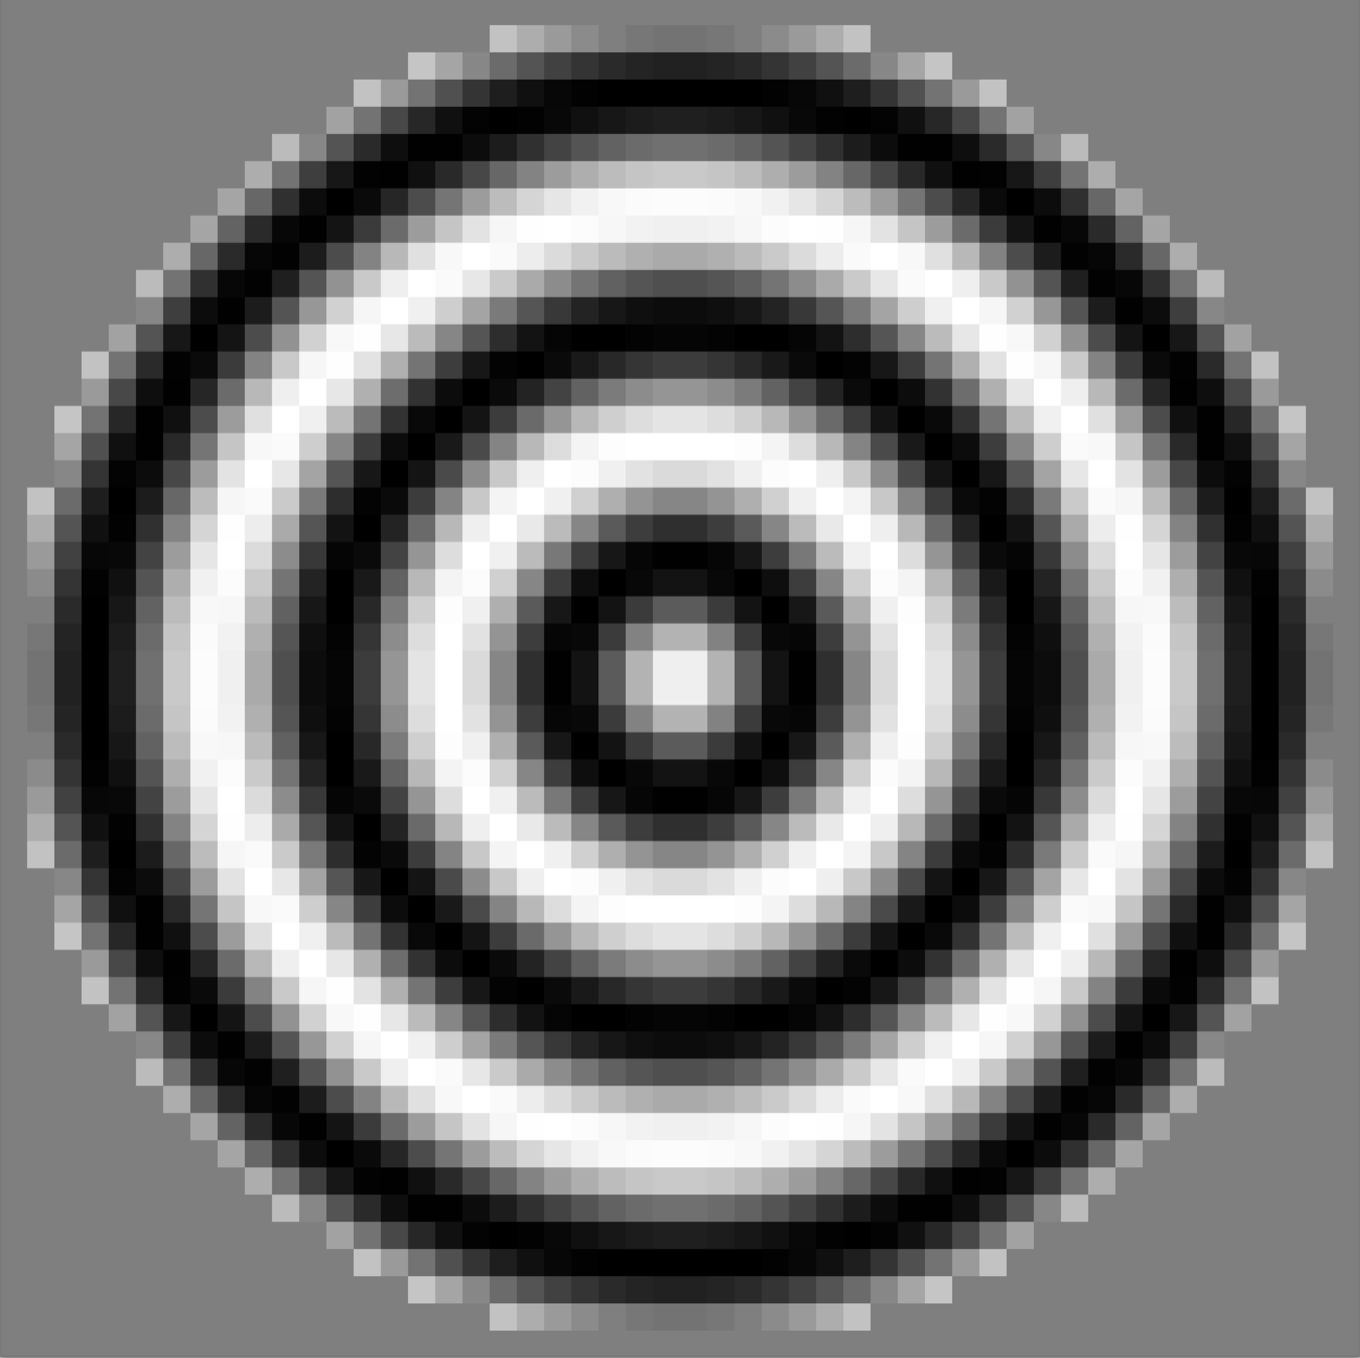
\includegraphics[width=0.2\textwidth]{assets/images/grating.png}
    \caption{An example of the annulus grating with maximal contrast and $\spatfreq = 5.7 \text{ cycles}/\circ, \vlum = 0.5, \diamdg = 0.7^\circ, \diam = 50$.}
    \label{fig:grating-example}
\end{figure}
\subsubsection{Figure composition}
\label{sec:figure-composition}

Let $\fullmatrix \in [0, 1]^{\fullwidth \times \fullheight}$ be the matrix allocated for the stimulus' luminance values, where $\fullwidth, \fullheight \in [\diam, \infty)$ represent the stimulus width and height, respectively.
Let $\figwidth \in (0, \frac{1}{2} \fullwidthdg]$ be the \stimfig{} width, and $\figheight \in (0, \frac{1}{2} \fullheightdg]$ - its height. The \stimfig{} comprises a submatrix of the full stimulus $\fullmatrix$. The \stimfig{} is located at the pixel distance $\figecc$ from the stimulus center, as defined in Equation (\ref{eq:figdiag}), at an angle $\figangle \sim U(\figanglemin, \figanglemax)$ to the horizontal axis. Since the \stimfig{} is located in the bottom right quadrant,
\begin{equation}
    \begin{aligned}
        \figanglemin &=
        \begin{cases}
            \cos^{-1} \left(
                \frac{\fullwidth - \figwidth}{2 \cdot \figecc}
            \right)
            &\text{ if } \figecc > \frac{\fullwidth - \figwidth}{2} \\
            \sin^{-1} \left( 
                \frac{\figheight}{2 \cdot \figecc}
            \right)
            &\text{ otherwise}
        \end{cases}, \\
        \figanglemax &= \frac{\pi}{2} - 
        \begin{cases}
            \cos^{-1} \left(
                \frac{\fullheight - \figheight}{2 \cdot \figecc}
            \right)
            &\text{ if } \figecc > \frac{\fullheight - \figheight}{2} \\
            \sin^{-1} \left( 
                \frac{\figwidth}{2 \cdot \figecc}
            \right)
            &\text{ otherwise}
        \end{cases}.
    \end{aligned}
\end{equation}
Now, we can locate the center of the \stimfig{} $\figcenter \in \mathbb{R}_+^2$:
\begin{equation}
    \figcenter = \left(
        \frac{1}{2} \fullwidth + \figecc \cdot \cos(\figangle), \
        \frac{1}{2} \fullheight + \figecc \cdot \sin(\figangle)
    \right).
\end{equation}
The center of the \stimfig{} need not be integer as it is only used for determining the \stimfig{}'s top left ($\figstart \in \mathbb{N}^2$) and bottom right ($\figfinish \in \mathbb{N}^2$) coordinates:
\begin{align}
\begin{split}
    \figstart &= \ceil{\figcenter - \frac{1}{2} (\figheight, \figwidth)}, \\
    \figfinish &= \figstart + (\figheight, \figwidth),
\end{split}
\label{eq:figure-location}
\end{align}
The ceiling function in Equation (\ref{eq:figure-location}) is applied element-wise.
\subsubsection{Annuli locations}
\label{sec:annuli-locations}

The distance between the centers of neighboring annuli is
\begin{equation}
    \anndist = \ceil{\anndistscale \cdot \diam}.
\end{equation}
The variable $\anndist \in \mathbb{N}$ then also indicates the number of pixels allocated to each annulus and void around it. Consequently, we can determine the number of annuli that are (partially) located in each row $\repsinrow \in \mathbb{N}$ and column $\repsincol \in \mathbb{N}$ of the stimulus:
\begin{equation}
    \repsinrow = \ceil{\frac{\fullwidth}{\anndist}}, \;
    \repsincol = \ceil{\frac{\fullheight}{\anndist}}. 
\end{equation}

Let $\annuliset$ be the set containing all matrices associated with annuli in $\fullmatrix$. Then, $|\annuliset| = \repsinrow \cdot \repsincol$, and
\begin{equation}
\begin{gathered}
    \annuliset \coloneqq \bigcup_{i = 0}^{\repsinrow - 1} \bigcup_{j = 0}^{\repsincol - 1}
    \begin{pmatrix}
        \fullmatrix_{\annstart_{\annuliset_{i, j}}} & & \\
         & \ddots & \\
         & & \fullmatrix_{\annfinish_{\annuliset_{i, j}}}
    \end{pmatrix}, \\
    \begin{aligned}
    \annstart_{\annuliset_{i, j}} &= \left( 
        i \cdot \anndist + \floor{ \frac{1}{2} (\anndist - \diam) }, \ 
        j \cdot \anndist + \floor{ \frac{1}{2} (\anndist - \diam) }
    \right), \\
    \annfinish_{\annuliset_{i, j}} &=
    \min(
        \annstart_{\annuliset_{i, j}} + (d, d), \ 
        (\fullwidth, \fullheight)
    ),
    \end{aligned}
\end{gathered}
\end{equation}
where $\annstart_{\annuliset_{i, j}}, \annfinish_{\annuliset_{i, j}} \in \mathbb{N}^2$ are the top left and bottom right coordinates of an annulus $\annuliset_{i, j} \in \annuliset$, respectively. 

As we position the annuli in the middle of the allocated space, for each stimulus, there exist values of $\anndistscale$, such that the last annulus in a row or column starts outside of the bounds of the figure. Such annuli need to be removed from the set $\annuliset$:
\begin{equation}
    \annuliset \leftarrow \annuliset \setminus \{ \annstimmatrix \in \annuliset \ | \ \annstart_\annstimmatrix > (\fullwidth, \fullheight) \}
\end{equation}
\subsubsection{Luminance assignment}
\label{sec:luminance-assignment}

First, all values of the stimulus $\fullmatrix$ are initialized with the void luminance $\vlum$. Then, the annuli with relevant contrasts are added to the matrix. Let $\view: \annuliset \to \{ \fig, \ground \}$ be the function mapping an annulus to its view. Let $\annstimmatrix \in \annuliset$, then
\begin{equation}
    \view(\annstimmatrix) = 
    \begin{cases}
        \fig & \text{ if } 
        \{ \annstart_\annstimmatrix, \cdots,  \annfinish_\annstimmatrix \}
        \cap
        \{ \figstart, \cdots, \figfinish \}
        \neq \emptyset \\
        \ground & \text{ otherwise} 
    \end{cases}.
\end{equation}
So, an annulus is said to be located in the figure if it is (partially) contained in it.

Let $\unirand: \annuliset \to U(0, 1)$ be a random value that varies per annulus. The values are independent and identically distributed (i.i.d.). Then for all $\annstimmatrix \in \annuliset$ and $\lambda, \mu \in \{ 0, 1, \cdots, \diam - 1\}, \ (i, j) = \annstart_\annstimmatrix + (\lambda, \mu)$,
\begin{equation}
    \fullmatrix_{i, j} \leftarrow \vlum +
    \begin{cases}
        (\annmatrix_{\lambda, \mu} - \vlum) \cdot \left( \unirand(\annstimmatrix) \contrange + \vlum \cdot (1 - \contrange) \right) 
        &\text{ if } \view(\annstimmatrix) = \fig  \\
        (\annmatrix_{\lambda, \mu} - \vlum) \cdot \unirand(\annstimmatrix) 
        &\text{ otherwise}
    \end{cases}.
\end{equation}
Now, the stimulus luminance matrix is complete.
Thus, the luminance of the void, similar to annuli's edges as demonstrated in Equation (\ref{eq:grating}), are still assigned the luminance of $\vlum$; the mean of all pixels' luminance values is also equal to $\vlum$. An example of the resulting luminance matrix' binary heat map is visualized in Figure \ref{fig:full-stimulus-example}.

\begin{figure}[!htp]
    \centering
    % ----- INPUT
\newcommand{\fsaimagew}{\textwidth}
\newcommand{\fsaimageh}{\fsaimagew}

% figure center
\newcommand{\fsafigcenterx}{0.68 * \fsaimagew}
\newcommand{\fsafigcentery}{0.2925 * \fsaimageh}

% figure dimensions
\newcommand{\fsafigw}{0.16 * \fsaimagew}
\newcommand{\fsafigh}{0.255 * \fsaimageh}

% patch dimensions
\newcommand{\fsapatchw}{0.1 * \fsaimagew}
\newcommand{\fsapatchh}{0.1 * \fsaimageh}

% shifts
\newcommand{\fsashiftw}{0.03 * \fsaimagew}
\newcommand{\fsashifth}{0.03 * \fsaimageh}

% ----- misc
\newcommand{\fsacenterx}{0.5 * \fsaimagew}
\newcommand{\fsacentery}{0.5 * \fsaimageh}

% figure coords
\newcommand{\fsafigleftx}{\fsafigcenterx - 0.5 * \fsafigw}
\newcommand{\fsafigrightx}{\fsafigcenterx + 0.5 * \fsafigw}
\newcommand{\fsafigtopy}{\fsafigcentery + 0.5 * \fsafigh}
\newcommand{\fsafigbottomy}{\fsafigcentery - 0.5 * \fsafigh}

% patch coords
\newcommand{\fsapatchleftx}{\fsafigcenterx - 0.5 * \fsapatchw}
\newcommand{\fsapatchrightx}{\fsafigcenterx + 0.5 * \fsapatchw}
\newcommand{\fsapatchtopy}{\fsafigcentery + 0.5 * \fsapatchh}
\newcommand{\fsapatchbottomy}{\fsafigcentery - 0.5 * \fsapatchh}

\begin{tikzpicture}[
        arr/.style = { -{Stealth[ ]} },
        whitedoublearrow/.style = {>=stealth, draw=white, fill=white, very thick, <->},
        pinkarrow/.style = {arr, draw=sec-color, fill=sec-color, very thick},
        yellowframe/.style = {rounded corners=0.2cm, very thick, main-color, fill=main-color, fill opacity=0.2},
        blueframe/.style = {rounded corners=0.2cm, very thick, third-color, fill=third-color, fill opacity=0.2},
        anglearrow/.style = {draw, >=stealth, white, very thick, ->, angle eccentricity=2}
    ]
    
    \begin{scope}
        \node[anchor=south west,inner sep=0] at (0,0) {
\includegraphics[width=\fsaimagew]{assets/images/full-stimulus.png}};
        
        % side length
        \node[] (startell) at (0, 0.95 * \fsaimageh) {};
        \node[] (endell) at (\fsaimagew, 0.95 * \fsaimageh) {};
        \path[whitedoublearrow, ultra thick] (startell) edge node {\bgcolorsmalltext{white}{black}{side length $\hat{\ell_\full}, ^\bigcirc$}} (endell);
        
        % center of gaze & stimulsus
        \node[style=cnode] (cent) at (\fsacenterx, \fsacentery) {};
        \node[shift={(-0.5 * \fsacenterx, 0)}] (centtxt) at (\fsacenterx, \fsacentery) {\bgcolorsmalltext{white}{black}{center of gaze \& stimulus $O_{L_\full}$}};
        \path [pinkarrow] (centtxt) edge[bend right=10] node {} (cent);
        
        % figure
        \node[shift={(0, \fsashifth)}] (figuretxt) at (\fsafigcenterx, \fsafigtopy) {\bgcolorsmalltext{white}{black}{figure $F$}};
        \draw[yellowframe] (\fsafigleftx, \fsafigtopy) rectangle (\fsafigrightx, \fsafigbottomy) {};
        
        % figure width
        \node[shift={(0, -1 * \fsashifth)}] (startfigw) at (\fsafigleftx, \fsafigbottomy) {};
        \node[shift={(0, -1 * \fsashifth)}] (endfigw) at (\fsafigrightx, \fsafigbottomy) {};
        
        \path[whitedoublearrow] (startfigw) edge node {\bgcolorsmalltext{white}{black}{$\hat{\ell_{F_w}}, ^\bigcirc$}} (endfigw);
        
        \draw[very thick, white] (\fsafigleftx, \fsafigbottomy) -- (\fsafigleftx, \fsafigbottomy - 2 * \fsashifth);
        \draw[very thick, white] (\fsafigrightx, \fsafigbottomy) -- (\fsafigrightx, \fsafigbottomy - 2 * \fsashifth);
        
        % figure height
        \node[shift={(\fsashiftw, 0)}] (startfigh) at (\fsafigrightx, \fsafigtopy) {};
        \node[shift={(\fsashiftw, 0)}] (endfigh) at (\fsafigrightx, \fsafigbottomy) {};
        
        \path[whitedoublearrow] (startfigh) edge node[rotate=90] {\bgcolorsmalltext{white}{black}{$\hat{\ell_{F_h}}, ^\bigcirc$}} (endfigh);
        
        \draw[very thick, white] (\fsafigrightx, \fsafigtopy) -- (\fsafigrightx + 2 * \fsashiftw, \fsafigtopy);
        \draw[very thick, white] (\fsafigrightx, \fsafigbottomy) -- (\fsafigrightx + 2 * \fsashiftw, \fsafigbottomy);
        
        % patch
        \node[shift={(0, \fsashifth)}] (patchtxt) at (\fsafigcenterx, \fsapatchtopy) {\bgcolorsmalltext{white}{black}{patch $L$}};
        \draw[blueframe] (\fsapatchleftx, \fsapatchtopy) rectangle (\fsapatchrightx, \fsapatchbottomy) {};
        
        % center of figure & patch
        \node[shift={(-0.3 * \fsaimagew, -0.1 * \fsaimageh)}] (cent2txt) at (\fsafigcenterx, \fsafigcentery) {\bgcolorsmalltext{white}{black}{center of figure \& patch $F_O$}};
        \node[style=cnode] (cent2) at (\fsafigcenterx, \fsafigcentery) {};
        \path [pinkarrow] (cent2txt) edge[bend right=10] node {} (cent2);
        
        % eccentricity
        \path[whitedoublearrow] (cent) edge node[sloped] {\bgcolorsmalltext{white}{black}{$\hat{\ecc_F}, ^\bigcirc$}} (cent2);
        
        % angle
        \draw[main-color] (\fsacenterx, \fsacentery) -- (\fsaimagew, \fsacentery);
        \node[] (xright) at (\fsaimagew, \fsacentery) {};
        \pic[anglearrow, "\bgcolorsmalltext{white}{black}{$\; \theta \;$}"] {angle = cent2--cent--xright};
        
        
    \end{scope}
\end{tikzpicture}
    \caption{An example of the full stimulus with parameters $ \spatfreq = 5.7 \text{ cycles}/\circ, \vlum = 0.5, \diamdg = 0.7^\circ, \diam = 48, \anndistscale = 1, \fullwidthdg = 33.87^\circ, \fullheightdg = 27.09^\circ, \contrange = 0.01, \figwidthdg = 5^\circ, \figheightdg = 9^\circ, \figeccdg = 11^\circ, \patchsizedg = 4.9^\circ$.}
    \label{fig:full-stimulus-example}
\end{figure}
\subsubsection{Patch selection}
\label{sec:patch-selection}

A square patch $\patchmatrix \in [0, 1]^{\patchsize \times \patchsize}$ is concentric to the figure $\figmatrix$. Thus, it can be defined as
\begin{equation}
    \patchmatrix \coloneqq 
    \begin{pmatrix}
        \fullmatrix_{\ceil{ \figcenter - \frac{\patchsize}{2}}, \ceil{  \figcenter - \frac{\patchsize}{2} }} &  &  \\
         & \ddots &  \\
         &  &  \fullmatrix_{\ceil{ \figcenter - \frac{\patchsize}{2}} + \ell, \ceil{  \figcenter - \frac{\patchsize}{2}} + \ell}
    \end{pmatrix}.
\end{equation}
An example of the resulting binary heat map of the texture stimulus patch is visualized in Figure \ref{fig:stim-patch-example}.

\begin{figure}
    \centering
    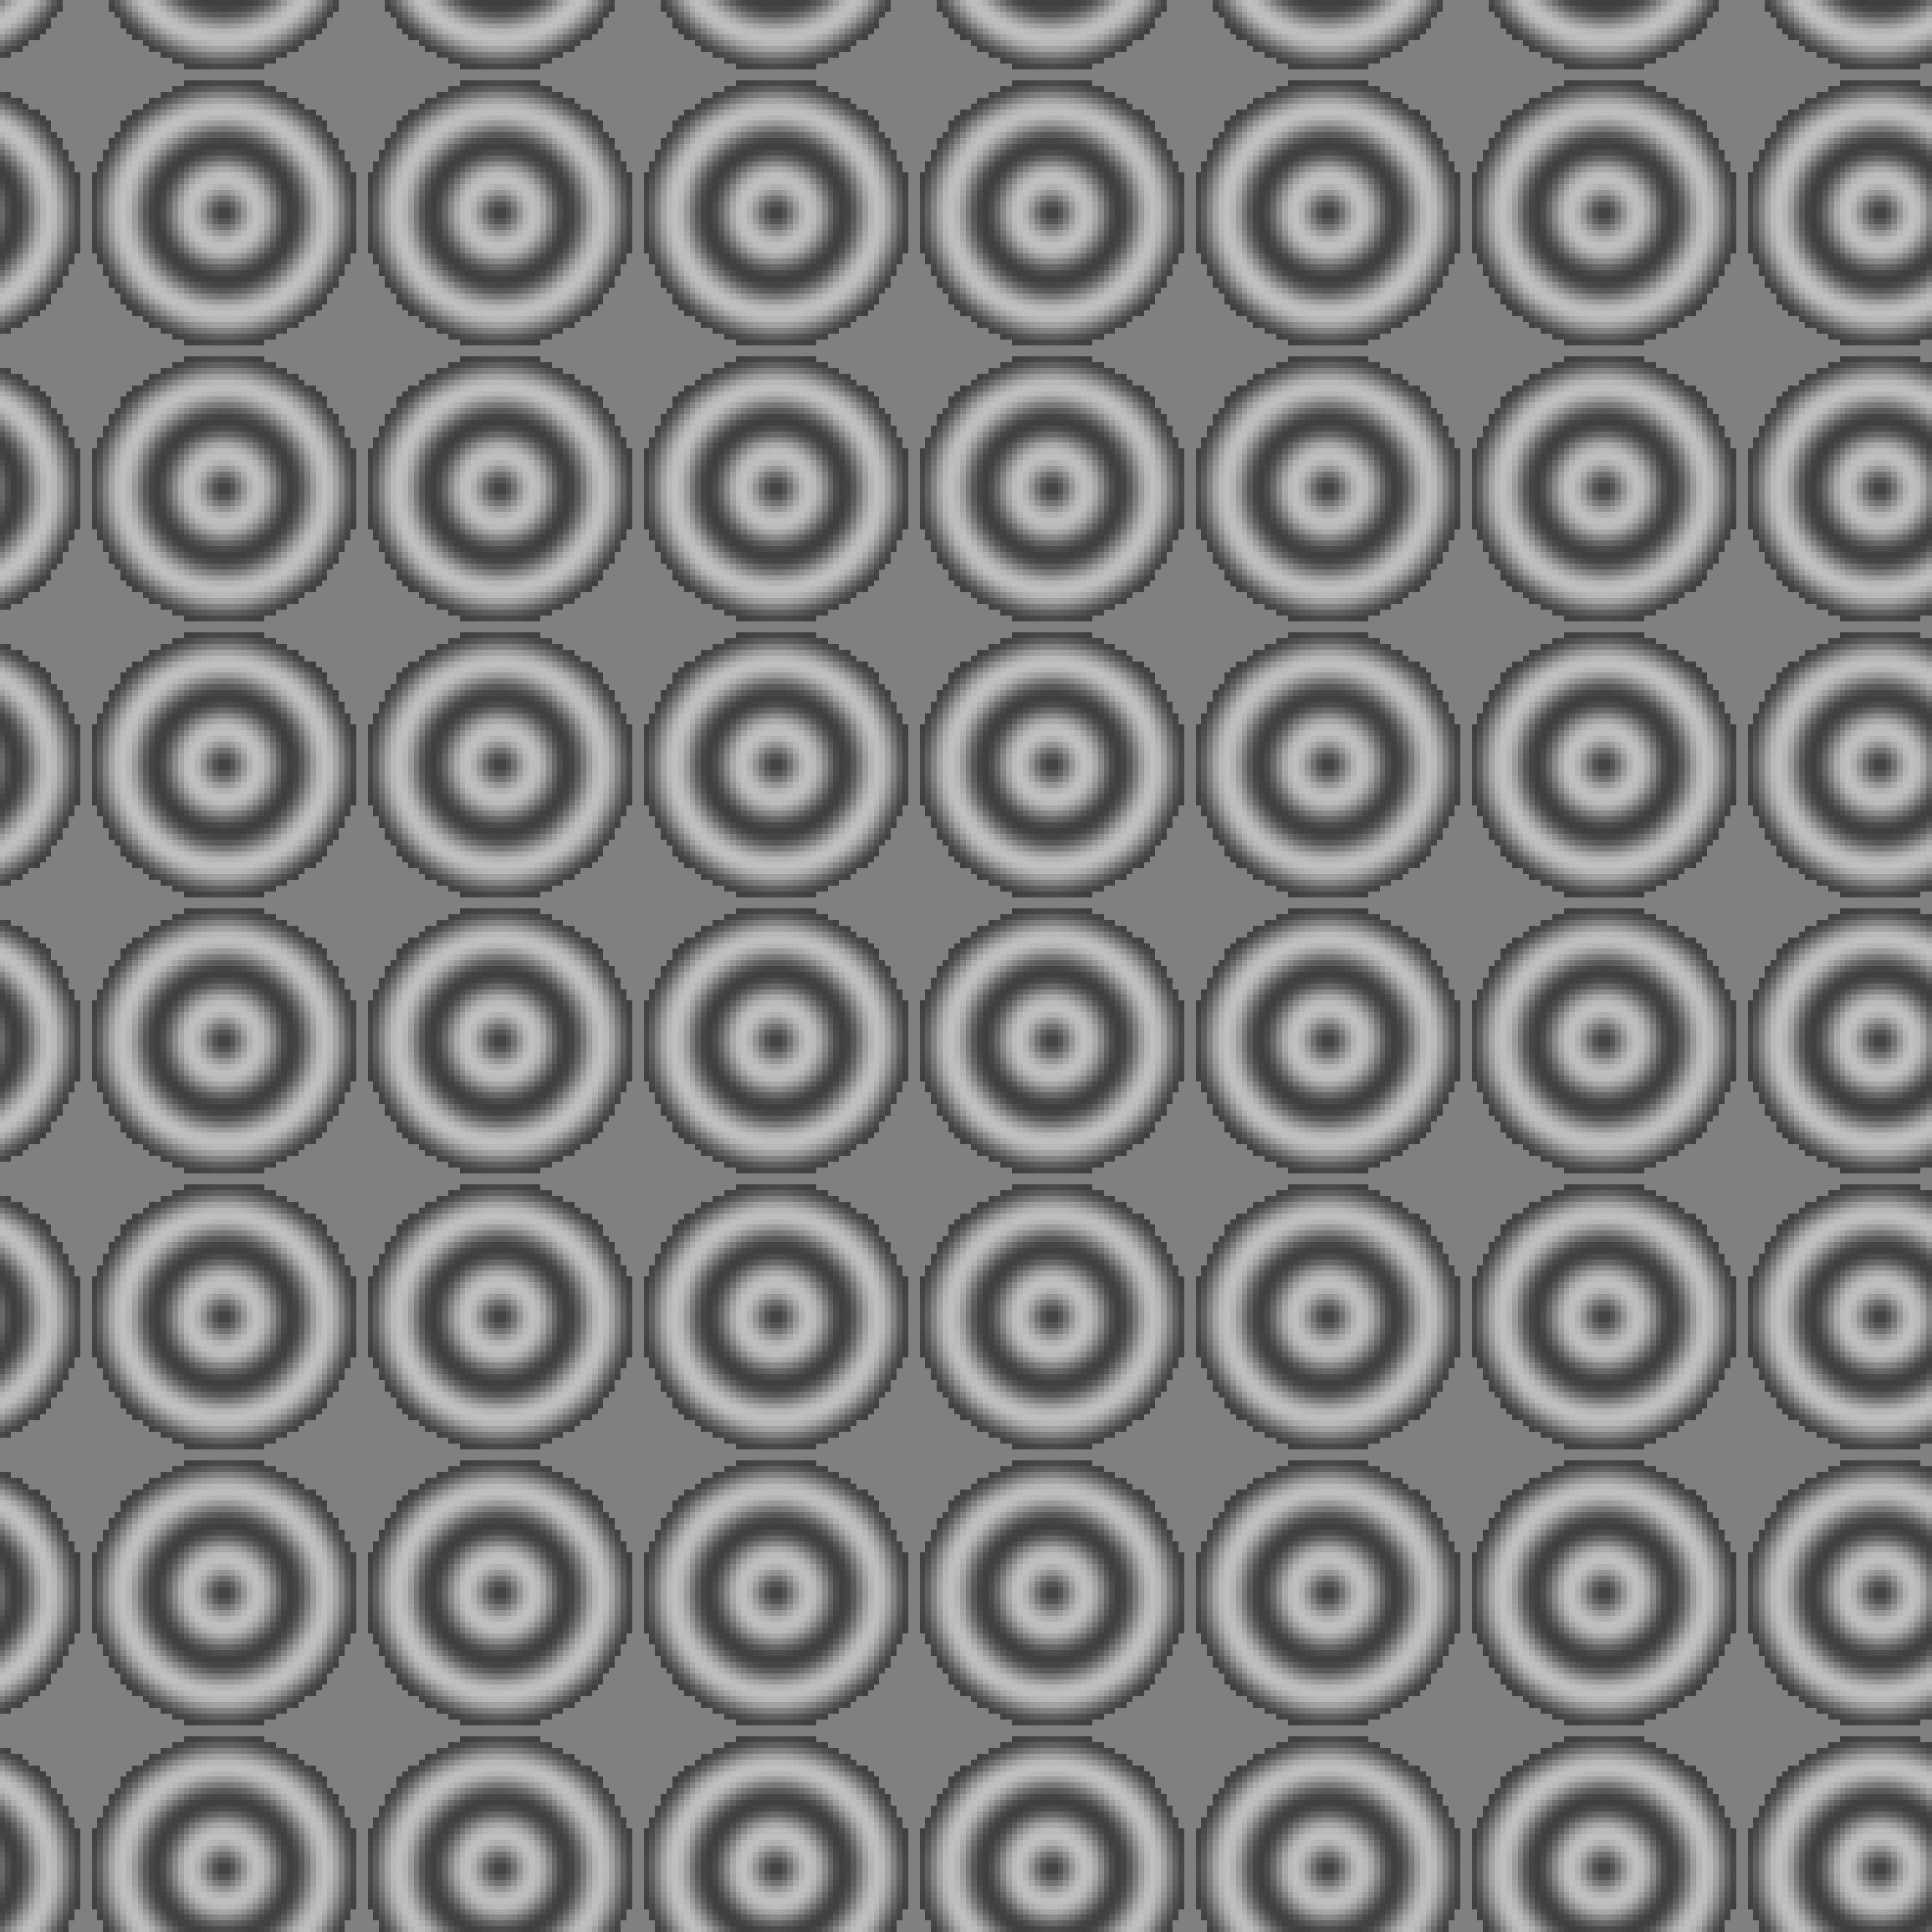
\includegraphics[width=0.4\textwidth]{src/assets/images/stimulus-patch.png}
    \caption{The stimulus patch obtained from Figure \ref{fig:full-stimulus-example}.}
    \label{fig:stim-patch-example}
\end{figure}






